\documentclass[border=3pt]{standalone}
\usepackage{xcolor}
\usepackage{tikz}
\usetikzlibrary{decorations.markings}

\begin{document}
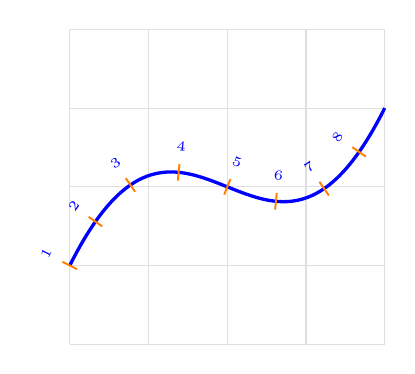
\begin{tikzpicture}[decoration={markings,
  mark=between positions 0 and 1 step .125 with {
    \draw[orange,line width=.7pt] (0,-3pt) -- (0,3pt);
    \node[font=\tiny,transform shape,above=4pt]
      {\pgfkeysvalueof{/pgf/decoration/mark info/sequence number}};}}]
  \draw[gray!25] (-2,-2) grid (2,2);
  \draw[blue,very thick,postaction={decorate}]
    (-2,-1) .. controls (-.5,2) and (.5,-2) .. (2,1);
\end{tikzpicture}
\end{document}
